\documentclass[border=10pt]{standalone}
\usepackage{pgfplots}
\pgfplotsset{compat=1.18}
\begin{document}
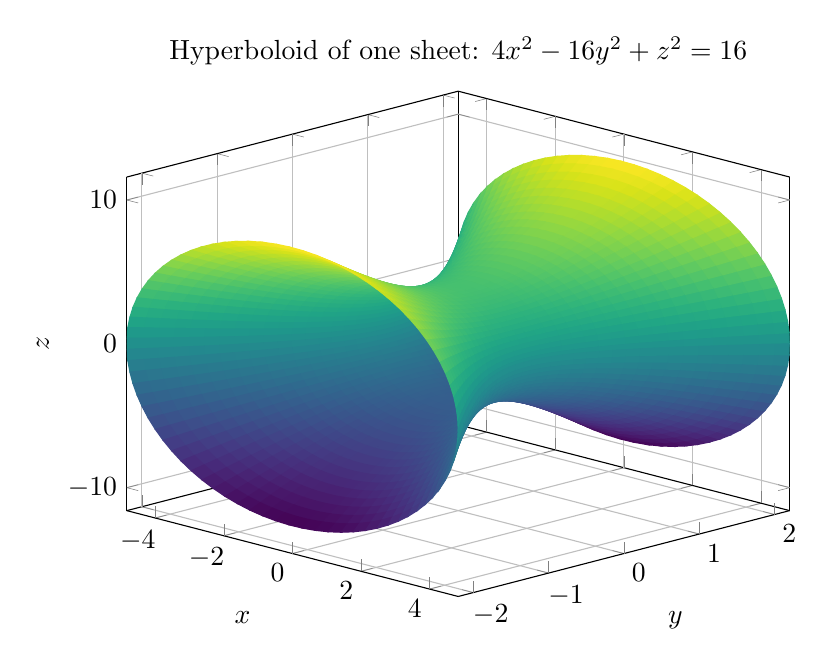
\begin{tikzpicture}
\begin{axis}[
    view={45}{20},
    xlabel={$x$}, ylabel={$y$}, zlabel={$z$},
    title={Hyperboloid of one sheet: $4x^2-16y^2+z^2=16$},
    grid=major,
    width=10cm, height=8cm,
    domain=0:2*pi, samples=80,
    y domain=-2.2:2.2, samples y=40,
    colormap/viridis
]
\addplot3[surf, shader=flat] ({2*sqrt(1+y^2)*cos(deg(x))}, y, {4*sqrt(1+y^2)*sin(deg(x))});
\end{axis}
\end{tikzpicture}
\end{document}